\documentclass[a4paper]{article}
\usepackage{amsmath,amssymb}
\usepackage{graphicx} % Required for inserting images
\usepackage{tikz}
\usepackage{hyperref}
\usepackage{cleveref}
\usepackage{pgfplots}
\usetikzlibrary{calc,arrows,shapes,positioning}
\usepackage{standalone}
\usepackage{subcaption}
\usepackage{booktabs}
\usepackage{siunitx} 
\usepackage{IAM_Lager}
\usepackage{float} 


\newtheorem{problem}{Problem}

\newcommand{\R}{\mathbb{R}}


\title{Optimization Methods for Sustainable Building Constructions}
\author{Stefan Martin Leiz, Valentin Fensterseifer}
\date{June 2026}

\begin{document}

\maketitle
\begin{abstract}

\end{abstract}


\tableofcontents
\clearpage
%%%%%%%%%%%%%%%%%%%%%%%%%%%%%%%%%%%%%%%%%%%%%%%%%%%%%%%%%%%%%%
\section{Parametric optimization of a two-span timber girder}
\begin{figure}[H]
    \centering
    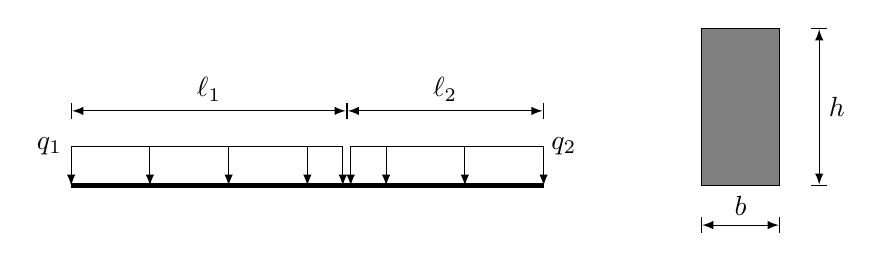
\begin{tikzpicture}[>=latex]
		\coordinate (A) at (0,0);
		\draw[ultra thick] (0,0) -- (6,0);
		\draw[|<->|] (0,0.95) -- ++(3.5,0.0) node[pos=.5,above]{$\ell_1$};
        \draw[|<->|] (3.5,0.95) -- +(2.5,0.0) node[pos=.5,above]{$\ell_2$};
		\foreach \x in {0,1,2,3,3.45,3.55,4,5,6}{
		\draw[<-] (\x,0) -- ++(0,0.5); };
		\draw[] (3.55,0.5) -- (6.0,0.5) node[pos=0.99,right]{$q_2$};
        \draw[] (0,0.5) -- (3.45,0.5) node[pos=0.001,left]{$q_1$};
		\Festlager{A};
		\Loslager{3.5,0}[0][1][0];
        \Loslager{6,0};
        \draw[fill=gray] (8,0) rectangle ++(1,2);
		\draw[|<->|] (8,-0.5) -- ++(1,0) node[pos=.5,above]{$b$};
		\draw[|<->|] (9.5,0.) -- ++(0,2) node[pos=.5,right]{$h$};
	\end{tikzpicture}	
    \caption{Mechanical system and cross-section of the parametric optimization of a two-span timber girder with field lengths $\ell_1$ and $\ell_2$.}
    \label{fig:beam}
\end{figure}
	 \begin{problem}\label{prob:timeber}
	     Given $\ell,\; q_d\in\R$. Find the optimal rectangular cross-section $(b,h)\in \mathbb R^2_+$ such that the used timber is minimized. Consider the bending, shear and deflection and other proofs.
    Furthermore, the width should not exceed $b_{max}\in\R_+$ and the height should not exceed $h_{max}\in\R_+$.
\end{problem}
\subsection{Objective function}

A mathematical formulation of \Cref{prob:timeber} reads: Find $(b,h)\in \mathbb R^2$ such that
	\begin{equation*}
		A(b,h) = b h  \rightarrow min,
	\end{equation*}
	subjected to the inequality constraints
	\begin{align*}
		g_{bending}(b,h) \le 0, \qquad g_{shear}(b,h) \le 0, \qquad
		g_{SLS}(b,h) \le 0,
	\end{align*}
	and the box-constraints
	\begin{align*}
	0\le b \le b_{max},\quad 0\le h \le h_{max}.
	\end{align*}

\subsection{Inequality constraints}
Here, we assume that the mechanics of the proofs are
	\begin{align*}
		g_{bending}(b,h) &= \tfrac{\tfrac{M_{max}}{W_y(b,h)}}{ k_{crit}(b,h)*f_{md}}-1  &&\mbox{with} \quad M_{max} = \tfrac{q_d\ell^2}{8}wrong,\\
		g_{shear}(b,h) &=\tfrac{\tfrac{3}{2}\tfrac{Q_{max}}{A(b,h)}}{f_{vd}}  - 1 &&\mbox{with} \quad Q_{max} = \tfrac{q_d\ell}{2}wrong,\\
		g_{SLS}(b,h) &= w_{max} - w_{adm}&&\mbox{with} \quad w_{max} = \tfrac{5}{384} \tfrac{ q_d  \ell^4}{E_{mean} Iy(b,h)}wrong.
	\end{align*}
\subsubsection{Sectional forces}


\subsubsection{Coefficients}
According to (Seite B.3/80) the overturning coefficient $k_{crit}$ is calculated by 
	\begin{align*}
		k_{crit}(b,h) = \begin{cases}
			1 \quad &\text{if \quad} \lambda_{rel,m} \leq 0.75\\
			1.56-0.75 \,\lambda_{rel,m} \quad &\text{if \quad} 0.75 < \lambda_{rel,m} \leq 1.4\\
			\frac{1}{\lambda_{rel,m}^2} \quad &\text{if \quad} 1.4 < \lambda_{rel,m},
		\end{cases}
	\end{align*}
where the relative lateral-torsional slenderness is
\begin{equation*}
	\lambda_{rel,m} = \sqrt{\frac{f_{m,k}}{\sigma_{m,crit}}} \qquad \mbox{with} \quad \sigma_{m,crit} = \frac{\pi\sqrt{E_{0.05}I_zG_{0.05}I_{tor}}}{\ell_\text{eff}{W_y}}.
\end{equation*}
%%%%%%%%%%%%%%%%%%%%%%%%%%%%%%%%%%%%%%%%%%%%%%%%%%%%%%%%%%%%%%
\newpage
\section{First ideas}
\begin{itemize}
    \item Example for a calculation of a timber beam ceiling with spacing between beams and a distributed area load
    \item the key verifications are shear, bending(lateral torsional buckling), deformation and maybe resonance test
    \item Include load combinations with inconvenient arrangement of use load
    \begin{itemize}
        \item simplification: $\ell_1 \ge \ell_2$
        \item either full load or use load only on l1

        \end{itemize}
\end{itemize}

\clearpage
\section{Example with values}
\begin{itemize}
    \item $\ell_1 = 5,0 m  $
    \item $\ell_2 = 3,0 m  $
    \item $g_k = 2,0 kN/m $
    \item $q_k = 3,0 kN/m $
    \item NKL1, C24, $k_mod = 0,8 $
    \item $b/h = 12/26 cm$

\end{itemize}

\end{document}
